% Two side document:\documentclass[12pt,a4paper,twoside]{report}
% Open right: \documentclass[12pt,a4paper,twoside,openright]{report}
\documentclass[12pt,a4paper,twoside,openright]{report}
\usepackage[T1]{fontenc} % Standard package for selecting font encodings
\usepackage{mathptmx} % Use Times as default text font, and provide maths 
%support
\usepackage{amsmath,amssymb,amsfonts} % for math typesetting
\usepackage{setspace} % Set space between lines
\usepackage[top=1in,bottom=1in,left=3.2cm,right=2.6cm]{geometry} % page style 
\usepackage{graphicx}\graphicspath{{img/}} % for images 
\usepackage{subcaption} % for subfigures 
\usepackage[sort&compress]{natbib} % for references 
\renewcommand{\bibname}{References} % Rename Bibliography to References 
\usepackage[hidelinks]{hyperref} % for hyperlinks 

% Fancy Headers: Extensive control of page headers and footers in LaTeX
\usepackage{fancyhdr}\pagestyle{fancy} 
\fancyhf{}
\fancyhead[RE]{\it{\nouppercase{\leftmark}}}
\fancyhead[LO]{\it{\nouppercase{\rightmark}}}
\fancyhead[LE,RO]{\thepage}
\fancyfoot{}

\usepackage{emptypage}
\usepackage[nottoc]{tocbibind}
\setcounter{secnumdepth}{3}
\setcounter{tocdepth}{3}

% Title Page 
\title{Report Writing using \LaTeX\\[1.5cm] 
\includegraphics[scale=0.6]{latex}}
\author{Author Name}
\date{Institute Name\\ Department Name\\[5mm] \today}

\raggedbottom

\begin{document}

\pagestyle{empty}	

\maketitle	
\cleardoublepage

\onehalfspacing
\pagenumbering{roman}
\pagestyle{plain}

% Abstract 
\begin{abstract}
An abstract is a brief summary of a research article, thesis, review, conference proceeding, or any in-depth analysis of a particular subject and is often used to help the reader quickly ascertain the paper's purpose.
\end{abstract}	

% Clear Page
\cleardoublepage
% Set Page Style 
\pagestyle{fancy}

% Table of Contents, List of Figures, List of Tables 
\tableofcontents
\listoffigures
\listoftables	

\cleardoublepage
\doublespacing
\pagenumbering{arabic}	

% Import Chapters
%================ch1======================================
\chapter{Introduction}\label{ch:ch1}

\section{A Little Intro to Bioinformatics and Genomics}
Genomics and Bioinformatics has become a buzzword in today's world of Science. About one or two decades ago, people saw biology and computer science as two different fields. One would learn about living beings and their functions whereas the other would learn about computers and underlying theories. However, at present, there seems to be a mere separation between two fields and this new-field, bioinformatics, has emerged as a combination of both Computer Science and Biology. And genomics is the study of genomes. Bioinformatics methods and tools are frequently used in genomics research, but genomics also makes use of many experimental methods. 

\section{Why Learn and Apply Genomics?} 
Bioinformatics and genomics have become an inter-disciplinary science and if you are a biologist, you will find that having knowledge in bioinformatics can benefit you immensely with your experiments and research.

A major application of bioinformatics can be found in the fields of \textbf{precision medicine}  and \textbf{preventive medicine}. Precision medicine consists of health care techniques customized for individual patients, including treatments and practices. Rather than treating or curing diseases, precision medicine focuses of developing measures to prevent diseases. Some of the diseases being focused are \textbf{influenza},\textbf{cancer}, \textbf{heart disease} and \textbf{diabetes}.


Researches are being carried out to identify genetic alterations in patients allowing scientists to come up with better treatments and even possible measures of prevention. Certain types of cancer, being caused by such genetic alterations can be identified beforehand and can be treated before the conditions get worse. \url{https://en.wikipedia.org/wiki/Genomics}


\section{What is Genome Analysis?} 
Modern biology is undergoing an historical transformation, becoming among other things increasingly data driven. A combination of statistical, computational, and biological methods has become the norm in modern genomic research. Of course this is at odds with the standard organization of university curricula, which typically focus on only one of these three subjects. It is hard enough to provide a good synthesis of computer science and statistics, let alone
to include molecular biology! Yet, the importance of the algorithms typical of this field can only be appreciated within their biological context, their results
can only be interpreted within a statistical framework, and a basic knowledge of all three areas is a necessary condition for any research project \cite{compgenome}.

Genome analysis, also known as genome mining or in silico analysis,currently constitutes an irreplaceable research tool for various aspects of microbiology\cite{ray2003}. In particular, the availability of genomes from virtually all bacterial human pathogens has opened perspectives in the fields
of diagnosis, epidemiology, pathophysiology and treatment.
A major advantage of genome sequences over phenotypic methods
is that data can rapidly be shared among scientists worldwide by being deposited in online databases and thus are easily comparable among laboratories.


\section{The Main Ideas}
The genomic sequencing era may be divided into two periods (Figure\ref{fig:sequencing_stats}). In the first decade, from 1995, when the sequencing of the \textit{Haemophilus influenzae} genome was performed \cite{ray2003} to 2005, sequencing relied on the classic Sanger method, was time- and money-consuming and was reserved to a limited number of sequencing centers world-wide. Fewer than 300 bacterial genomes were sequenced during this period (Figure\ref{fig:sequencing_stats}). Since 2005, the development of new and high-throughput sequencing methods,2 together with a steep decrease of the sequencers’ and reagents’ cost enabling many laboratories to develop their own sequencing projects, led to a striking increase in the number of sequenced genomes, approaching 6000 for the year 2013 alone. The tremendous source of information provided by genome sequences revolutionized basic aspects of microbiology. In particular,genome sizes of bacteria range from 139 kb for Candidatus Tremblaya princeps to 14 782 kb for Sorangium cellulosum (\url{http://genomesonline.org/})  \cite{ray2003}


With more than 49 000 bacterial genome sequences currently available,including those from all significant human pathogens, genomics has a significant impact on clinical microbiology and infectious diseases by enabling the development of improved diagnostic, genotyping, taxo-nomic, antibiotic and virulence marker detection tools as well as development of new culture media or vaccines. This chapter summarizes the current achievements in bacterial genomics relevant to medical microbiology.

\begin{figure}
	\centering
	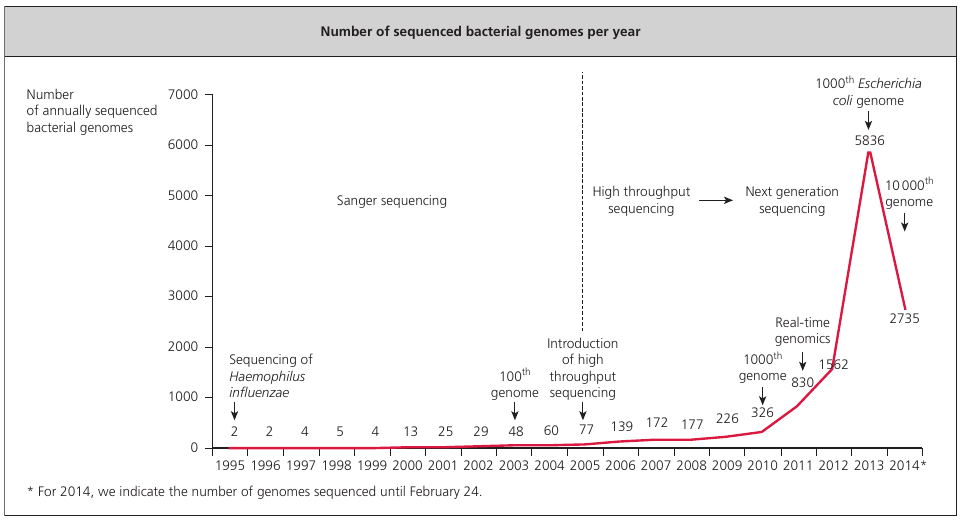
\includegraphics[width=\linewidth]{sequencing_stats}
	\caption{ Number of sequenced bacterial genomes per year.}
	\label{fig:sequencing_stats}
\end{figure} 

\section{Genomic Approaches}
The ultimate goal of genetic association studies is both to define the genetic architecture of complex traits and diseases and also to provide new insights into normal physiology and disease pathophysiology. Accomplishing that goal will require defining the causal variants that account for the observed associations, their mechanism of action, and their target genes. Success would have both near- and long-term benefits to health and science. In terms of health benefits, causal relationships between noncoding genetic variants and disease risk can be used to improve the prediction of disease onset and the design of prevention and early detection strategies. Subsequently determining the effects of causal variants on gene expression can prioritize downstream efforts to characterize causal genes and their role in disease etiology. That prioritization is particularly valuable when the target genes have an unknown function. This discovery pathway can ultimately lead to novel and potentially patient-specific therapeutic targets. In terms of scientific benefits, expanding the catalog of noncoding variants that are known to contribute to human traits is needed to determine general and transferrable principles about the genetic basis of complex human diseases. Recent conceptual and technical advances in genetics and genomics together have the potential to greatly improve our understanding of the noncoding genetic contributions to human traits. Although there are a wide variety of ways in which noncoding variants may affect phenotypes, we will focus specifically on variants that alter the activity of gene regulatory elements and, subsequently, the expression of target genes\cite{lowe2015genomic}.

% Chapter-2
\chapter{Literature}\label{ch:ch2}
Lorem Ipsum is simply dummy text of the printing and typesetting industry. 
Lorem Ipsum has been the industry's standard dummy text ever since the 1500s, 
when an unknown printer took a galley of type and scrambled it to make a type 
specimen book. It has survived not only five centuries, but also the leap into 
electronic typesetting, remaining essentially unchanged\cite{Prjibelski2018}. 
It was popularised in 
the 1960s with the release of Letraset sheets containing Lorem Ipsum passages, 
and more recently with desktop publishing software like Aldus PageMaker 
including versions of Lorem Ipsum.

\section{Equation}
Lorem Ipsum is simply dummy text of the printing and typesetting industry. 
Lorem Ipsum has been the industry's standard dummy text ever since the 1500s, 
when an unknown printer took a galley of type and scrambled it to make a type 
specimen book. It has survived not only five centuries, but also the leap into 
electronic typesetting, remaining essentially unchanged. It was popularised in 
the 1960s with the release of Letraset sheets containing Lorem Ipsum passages, 
and more recently with desktop publishing software like Aldus PageMaker 
including versions of Lorem Ipsum.\cite{Land2015} 

The velocity, v ($v=d/t$) is ....

\begin{equation}
\nu = \frac{\mu}{\rho}
\end{equation}

\begin{table}
\centering
\caption{Random table-2}
\label{tab:sample2}
\begin{tabular}{|c|c|c|c|c|c|c|c|c|c|}
\hline 
a & b & c & d & b & c & d & b & c & d \\ \hline 
5 & 6 & 7 & 8 & b & c & d & b & c & d\\ \hline 
9 & 10 & 11 & 12 & b & c & d & b & c & d \\ \hline 
a & b & c & d & b & c & d & b & c & d\\ \hline 
5 & 6 & 7 & 8 & b & c & d & b & c & d\\ \hline 
9 & 10 & 11 & 12 & b & c & d & b & c & d \\ \hline 
a & b & c & d & b & c & d & b & c & d\\ \hline 
\end{tabular} 
\end{table}          	
%================ch3======================================
\chapter{Genomics Application}\label{ch:ch3}

\section{Role of Genomics in Clinical Microbiology} 
There are multiple applications for genomics in clinical
microbiology\cite{ray2003}. 
\begin{itemize}
	\item  Real-time genomics may be used to investigate infectious disease outbreaks
	\item  Bacterial genomes may be used as target sources for molecular detection, identification or genotyping.
	\item The gene content, obtained by comparison to databases such as Clusters of Orthologous Groups (\url{www.ncbi.nlm.nih.gov/COG/}) or Kyoto Encyclopedia of Genes and Genomes (\url{www.genome.ad.jp/kegg/}), may be searched for specific phenotypic traits such as virulence or antibiotic resistance markers, or deficient metabolic pathways enabling design of improved culture media.
	
	\item Antigenic epitopes detected in the deduced proteome may be
	used for serologic applications, development of monoclonal
	antibodies or development of vaccines (Figure~\ref{fig:genome}).
	\item Taxonomic description of new bacterial species.
\end{itemize}

\begin{figure}
	\centering
	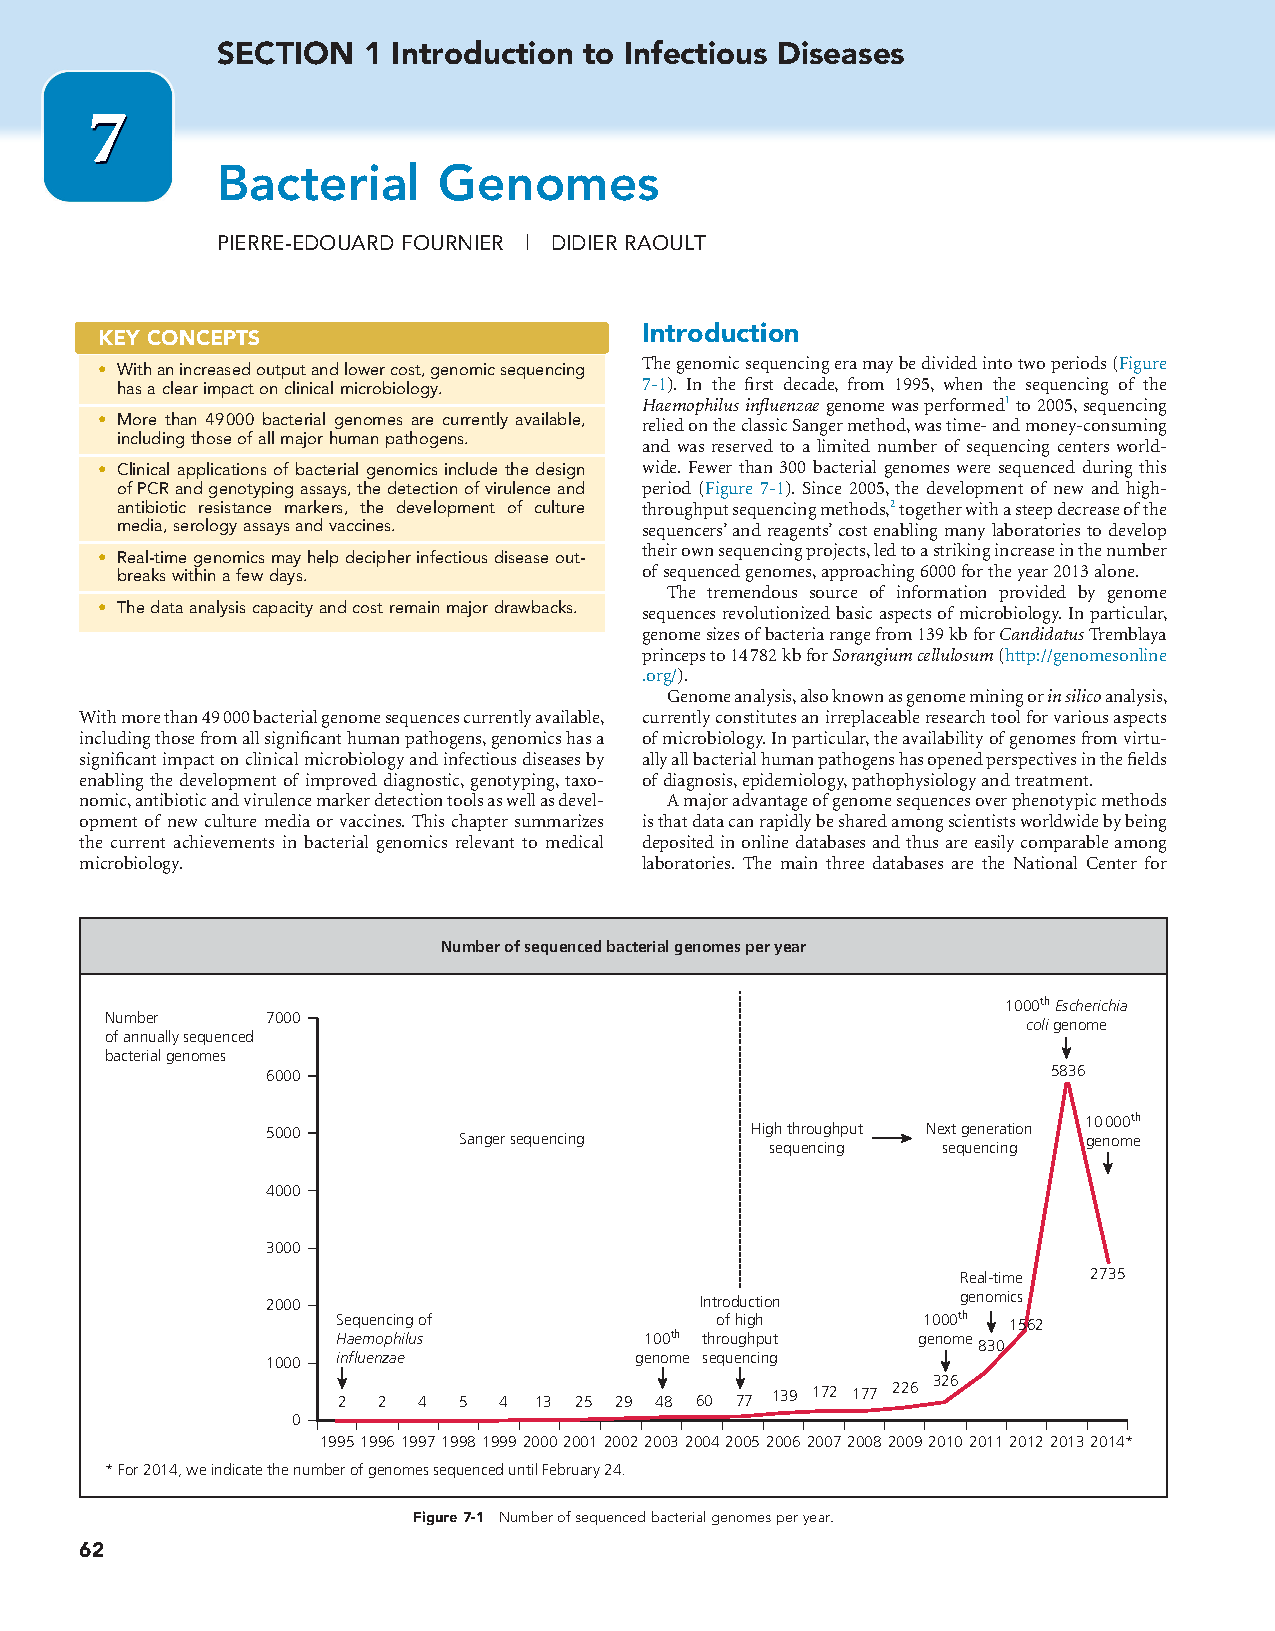
\includegraphics[width=0.9\linewidth]{backterial_genome}
	\caption{Applications of genomics to the clinical microbiology laboratory.}
	\label{fig:genome}
\end{figure} 


\section{The Clinical Applications of Genomic Technologies}
The clinical applications of genomic technologies are vast and offer opportunities to improve healthcare across the breadth of medical specialities. I will explore some of these applications in more depth this section.

\subsection{Gene discovery and diagnosis of rare monogenic disorders} 
Genomic technologies can be used by clinicians from all specialities to diagnose their patients who have high-risk genetic errors causing disease. Researchers are using these techniques to identify new genes which cause genetic disease at an astonishing rate - over 4000 diseases now have a known single genetic cause, compared to around 50 in 1990.

\subsection{Identification and diagnosis of genetic factors contributing to common disease} 
Genomic technologies are increasingly being used to understand the contribution of both rare and common genetic factors to the development of common diseases, such as high blood pressure, diabetes and cancer.

\subsection{Pharmacogenetics and targeted therapy}
Genetic information may be used to predict whether a person will respond to a particular drug, how well they will respond to that drug and whether they are likely to get any side effects from the use of a specific drug. This allows their treating team to make individualised decisions about the right drug treatment. In some cases, such as cancer, we can identify the genetic drivers of disease and then give drugs which specifically target that pathway. This is known as targeted therapy.

\subsection{Prenatal diagnosis and testing}
Genetic diseases are often devastating and may cause significant disability and even death in childhood. Prenatal diagnosis of genetic diseases allows parents to make decisions about whether to continue with the pregnancy or to allow early diagnosis and possible treatment in utero or at birth. Whilst previous approaches to prenatal diagnosis could put the pregnancy at risk, new methods using genomic technology can look directly at the DNA of the fetus from a maternal blood test, without increasing the risk of miscarriage - this is known as non-invasive prenatal testing. The use of NGS and array technology in prenatal samples is also on the increase to improve diagnostic yields in a pregnancy.

\subsection{Infectious diseases} 
Sequencing the genomes of microorganisms which cause human infection can identify the exact organism causing symptoms, help to trace the cause of infectious outbreaks, and give information as to which antibiotics are most likely to be effective in treatment.


\subsection{Personalised medicine}
As the exact DNA sequence of the genome of each human is unique to them, we will all have unique disease susceptibilities and treatment responses. Personalised medicine describes the use of our genetic information to tailor health care intervention to our own individual need.

\subsection{Gene therapy}
Gene therapy involves the administration of DNA or RNA, in order to correct a genetic abnormality, or modify the expression of genes.

\subsection{Genome editing}
Genome editing uses molecular techniques to modify the genome - genome editing can add in, cut out, or replace sections of the DNA sequence.

\subsection{Design of new antimicrobial agents and vaccines}
One of the expected benefits of genome analysis of pathogenic bacteria is in the area of human health, particularly in the design of more rapid diagnostic reagents and the development of new vaccines and antimicrobial agents. These goals have become more urgent with the continuing spread of antibiotic resistance in important human pathogens. Moreover, results from the whole-genome analysis of human pathogens has suggested that there are mechanisms for generating antigenic variation in proteins expressed on the cell surface that are encoded within the genomes of these organisms\cite{fraser2000microbial}.
These mechanisms include the following:

\begin{enumerate}
	\item slipped-strand mispairing
	within DNA sequence repeats found in 58-intergenic regions and coding sequences as described for \textit{H. influenzae2} \textit{ Helicobacter pylori26}  and \textit{M. tuberculosis27} 
	
	\item recombination between homologous genes
	encoding outer-surface proteins as described for Mycoplasma
	genitalium28, Mycoplasma pneumoniae29 and Treponema pallidum30 (Figure~\ref{fig:vac})
	
	\item clonal variability in surface-expressed proteins as described for Plasmodium falciparum31 and possibly Borrelia burgdorferi32. \cite{fraser2000microbial}
	
\end{enumerate} 

\begin{figure}
	\centering
	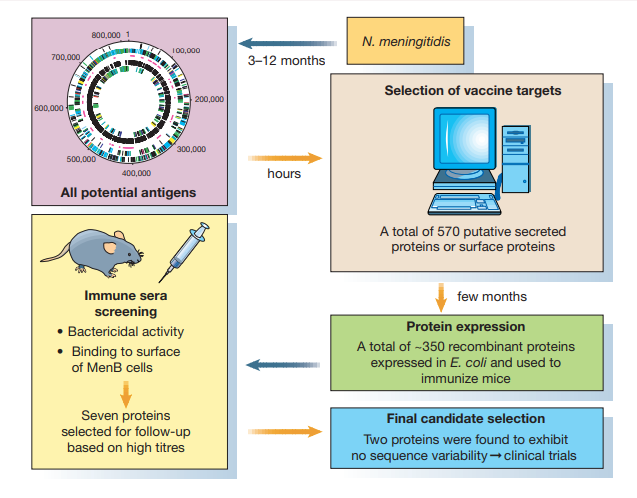
\includegraphics[width=0.9\linewidth]{vaccine}
	\caption{ Diagram depicting how complete microbial genome sequence data can accelerate vaccine development.}
	\label{fig:vac}
\end{figure} 

	

% Import Appendix 
\appendix	
%%================app1======================================
\chapter{Supporting Information}\label{app:app1}

\begin{figure}[h]
	\centering
	\includegraphics[width=.5\textwidth]{image2}
	\caption{Caption of image 2.}
	\label{fig: img2}
\end{figure}	

\singlespacing

% Import BibTeX
% Bibliographystyle: plain, abbrv, acm, 
\bibliographystyle{plain}	
\bibliography{references}
	
\end{document}